%% Meghan Sullivan
%% 20180219
%% Git Slides

\documentclass[border=15pt]{standalone}

\usepackage{tikz}

\tikzset{
	% Two node styles for game trees: solid and hollow
	solid node/.style={circle,draw,inner sep=1.5,fill=black},
	hollow node/.style={circle,draw,inner sep=1.5}
}


\begin{document}

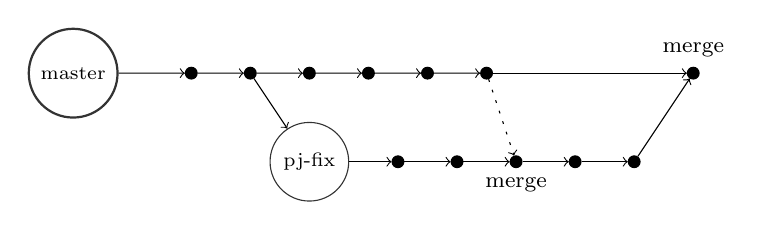
\begin{tikzpicture}[scale=1.5,font=\footnotesize]

% set top (root) node (level 1)
\node[shape=circle, draw = black!80, thick, font=\scriptsize] (m) at (0, 0.75)  {master};
\node(1) at (1, 0.75) [solid node] {};
\node(2) at (1.5, 0.75) [solid node] {};
\node(3) at (2, 0.75) [solid node] {};
\node(4) at (2.5, 0.75) [solid node] {};
\node(5) at (3, 0.75) [solid node] {};
\node(6) at (3.5, 0.75) [solid node] {};
\node(12) at (5.25, 0.75) [solid node, label = above:merge] {};

\node[shape=circle, draw=black!80, thin, font=\scriptsize] (branch) at (2, 0) {pj-fix};
\node(7) at (2.75, 0) [solid node] {};
\node(8) at (3.25, 0) [solid node] {};
\node(9) at (3.75, 0) [solid node, label = below:merge] {};
\node(10) at (4.25, 0) [solid node] {};
\node(11) at (4.75, 0) [solid node] {};

\path[->] (m) edge (1)
          (1) edge (2)
          (2) edge (3)
          (2) edge (branch)
          (3) edge (4)
          (4) edge (5)
          (5) edge (6)
          (branch) edge (7)
          (7) edge (8)
          (8) edge (9)
          (9) edge (10)
          (10) edge (11)
          (11) edge (12)
          (6) edge (12);
\path[->, dash pattern=on 1pt off 3pt] (6) edge (9);

\end{tikzpicture}

\end{document}
